\chapter{Calibration}
\label{sec:calib}
\section{$\ce{^{16}N}$}
The accuracy of simulated events is evaluated with data taken while a
radioactive source was deployed within the detector volume.
The data taken with the source deployed is used to assign systematics to reconstructed
values and, in the case of the energy reconstruction, determine an empirical
correction to improve the agreement between detected and MC simulated events.
For this analysis an $\ce{^{16}N}$ source was used.
The SNO+ $\ce{^{16}N}$ source was developed for SNO, as
their primary energy calibration source~\citep{sno_n16}.
The methods and results of SNO+'s $\ce{^{16}N}$ calibration are summarized here but
are described in greater detail by~\citep{snop_water_unidoc}.

\begin{figure}[htbp]
\centering
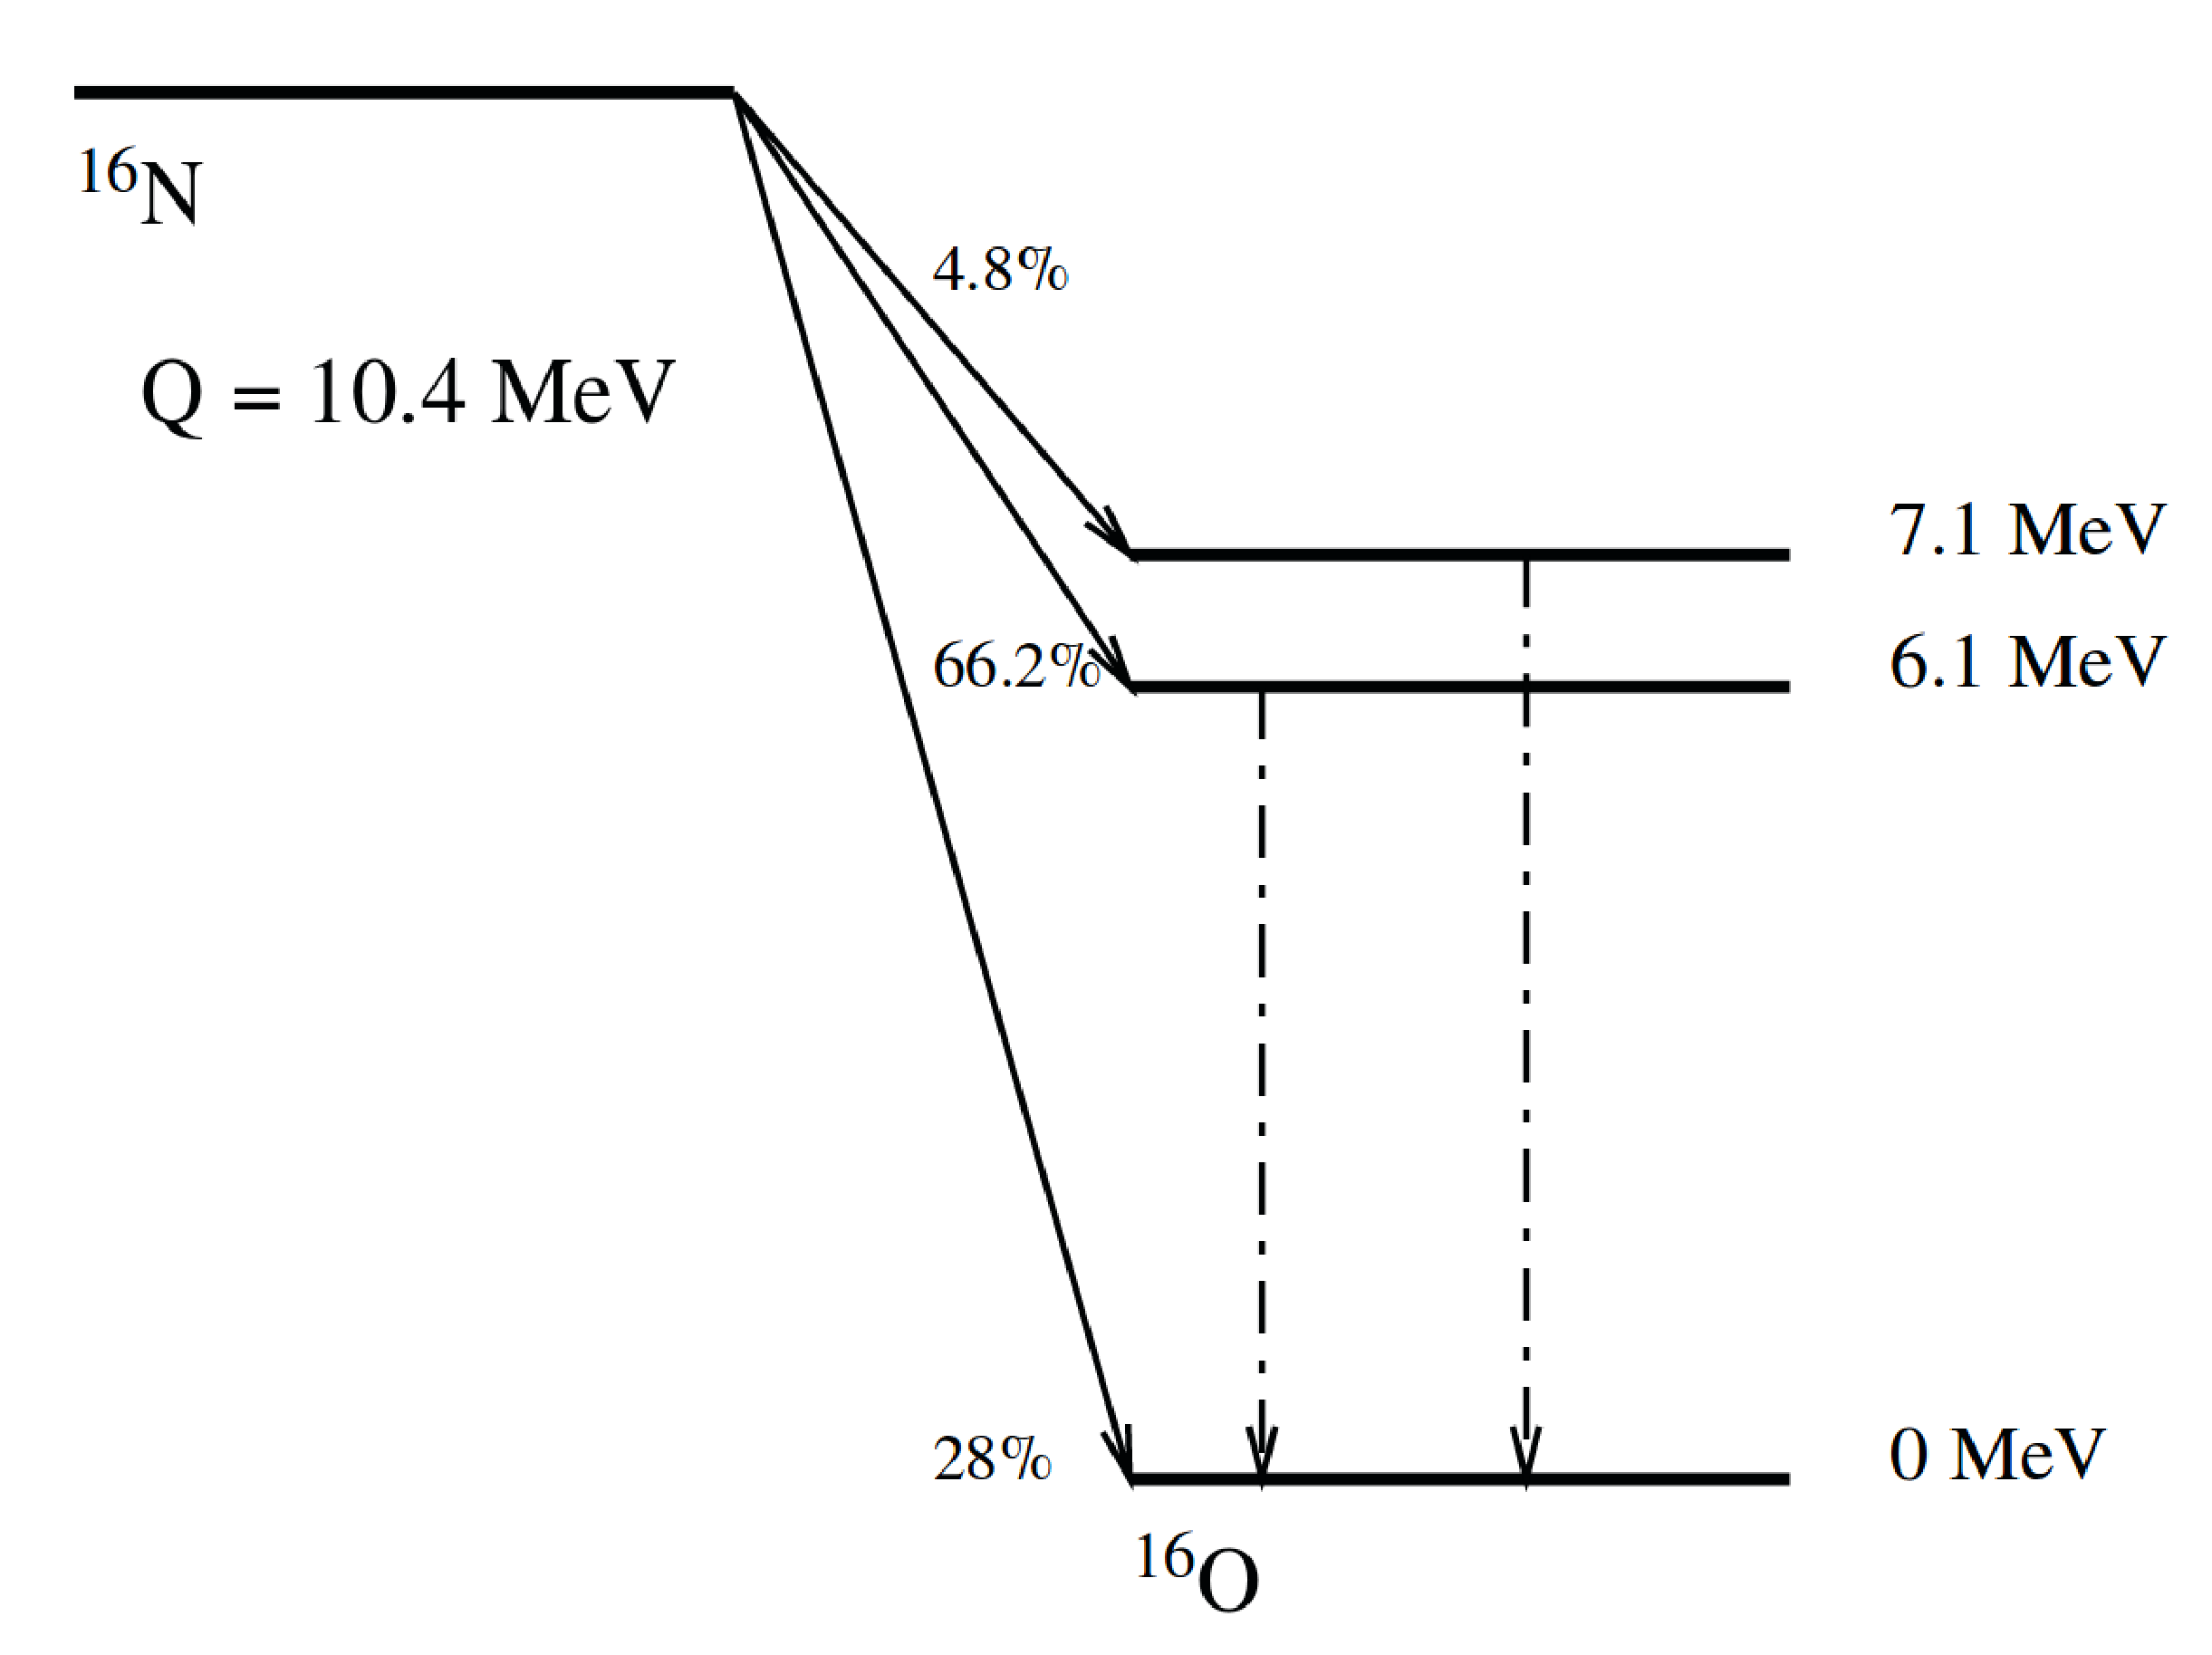
\includegraphics[width=0.58\textwidth]{n16_branching_ratios}
\caption[Major $\ce{^{16}N}$ Branching Ratios]{The most significant branching ratios for $\ce{^{16}N}$ decaying
to an excited state of $\ce{^{16}O}$. Figure from~\citep{sno_n16}.}
\label{fig:n16_br}
\end{figure}
The $\ce{^{16}N}$ source uses a commercial
deuterium and tritium generator (DT-generator) to produce gaseous $\ce{^{16}N}$.
The gas is pumped into the deployed source where it can undergo $\beta$-decay
to an excited state of $\ce{^{16}O}$, the $\ce{^{16}O}$ will then de-excite
and typically emit a $6.1$\,MeV gamma particle. Higher or lower energy gammas are emitted
at a lower rate, the primary branching ratios for the de-excitation gammas are shown in
Fig~\ref{fig:n16_br}.

A small block of plastic scintillator, observed by a PMT, is embedded within the
source cannister. The PMT detects the $\beta$ from the initial
$\ce{^{16}N} \rightarrow \ce{^{16}O^{*}}$ decay. That PMT signal is used as a
tag in the detector DAQ to identify events from the deployed source.

The source position within the AV was varied in a 3-dimensional
scan.
A 1-dimensional scan was done along the z-axis between the AV and PSUP\@.
Scanning many positions allowed for a position dependent evaluation of
systematics and a position dependent correction to the reconstructed energy.
The analyses that were done using $\ce{^{16}N}$ data to constrain systematics
relevant to the solar neutrino analysis are discussed in Sec~\ref{sec:systematics}.

\section{Trigger Efficiency}
\label{sec:trigeff}
\begin{figure}[htbp]
    \centering
    \begin{subfigure}{0.78\textwidth}
        \centering
    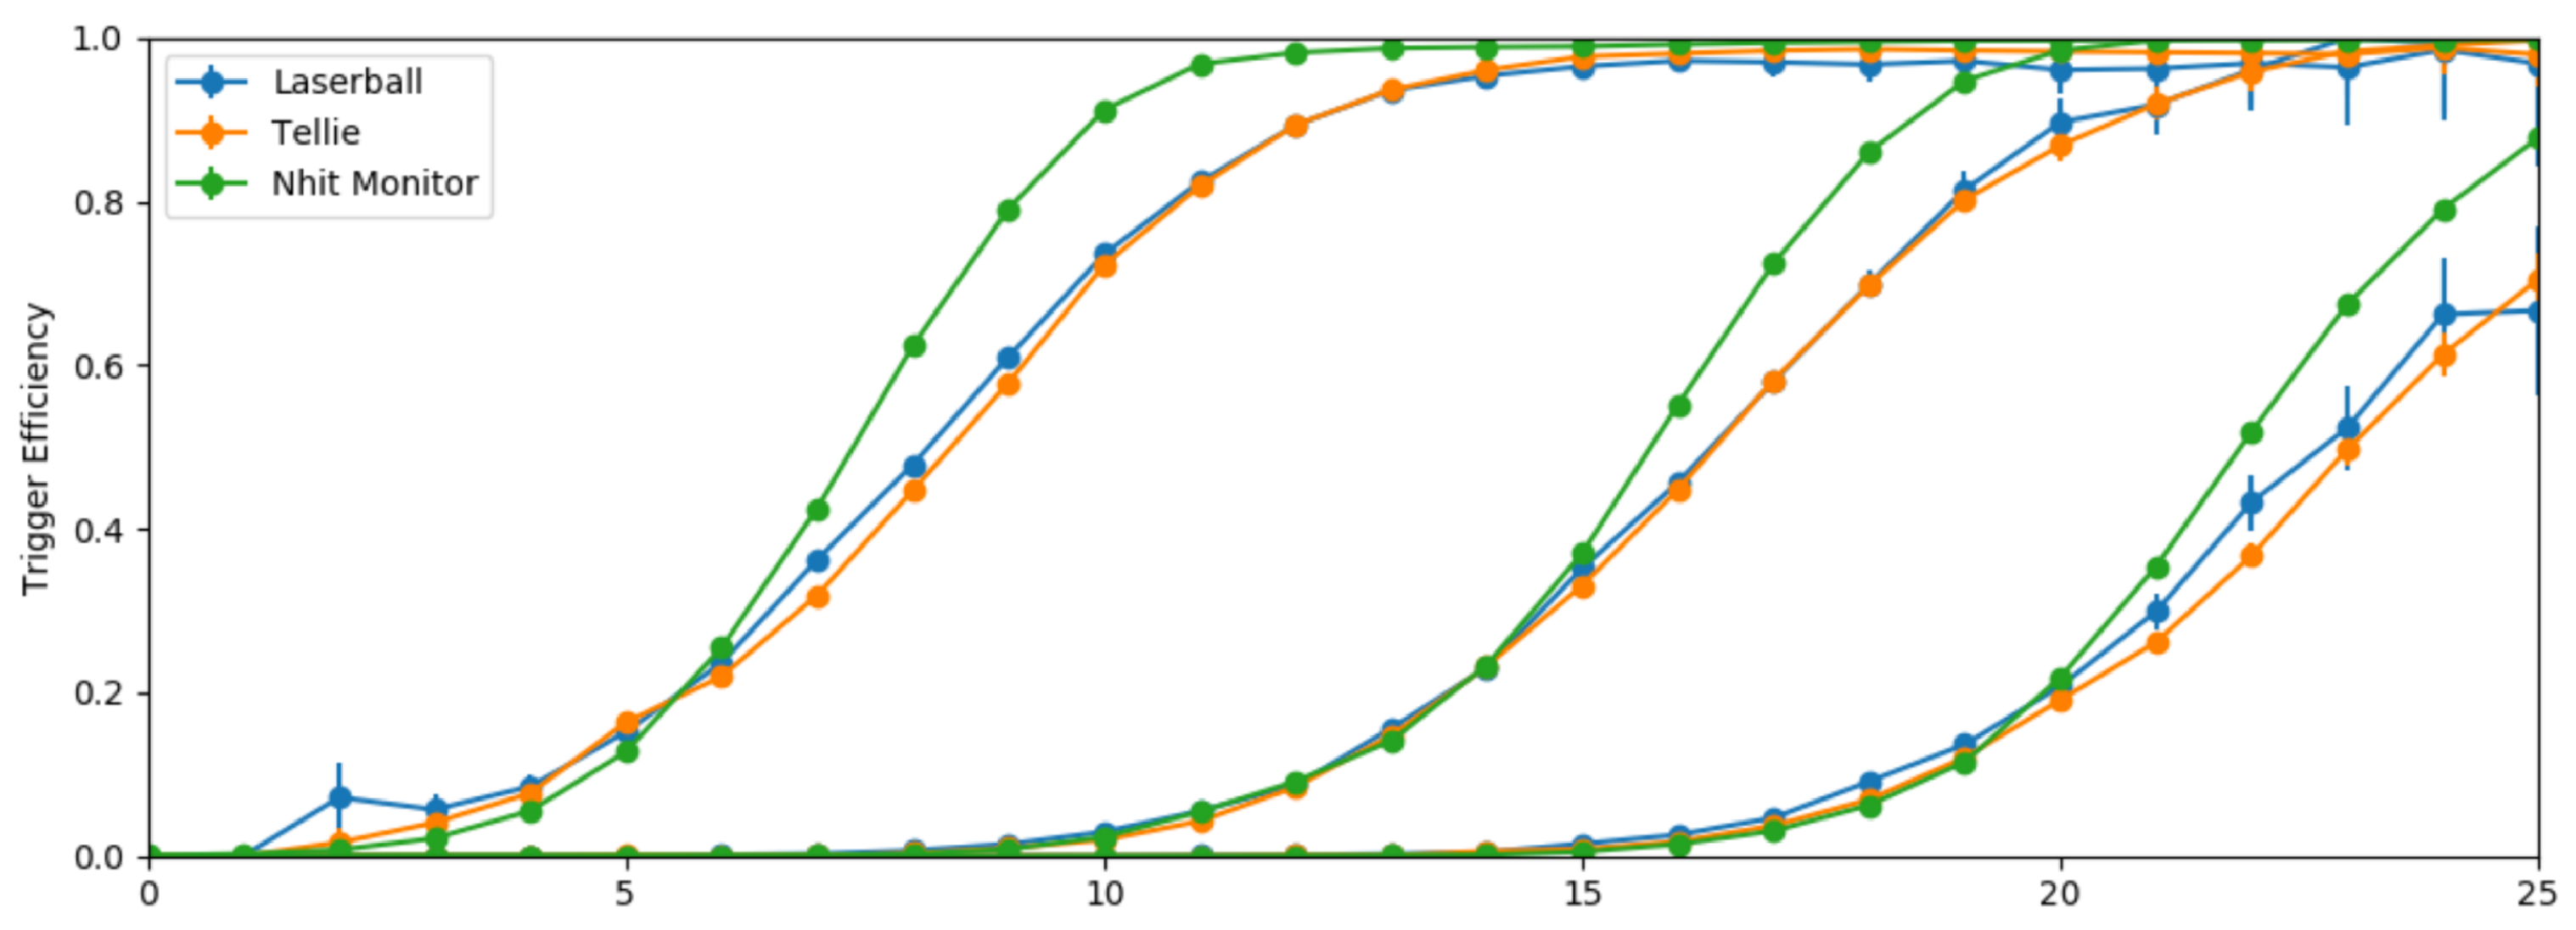
\includegraphics[width=\textwidth]{trigger_eff_plot}
    \caption{}
    \end{subfigure}
    \begin{subfigure}{0.78\textwidth}
        \centering
    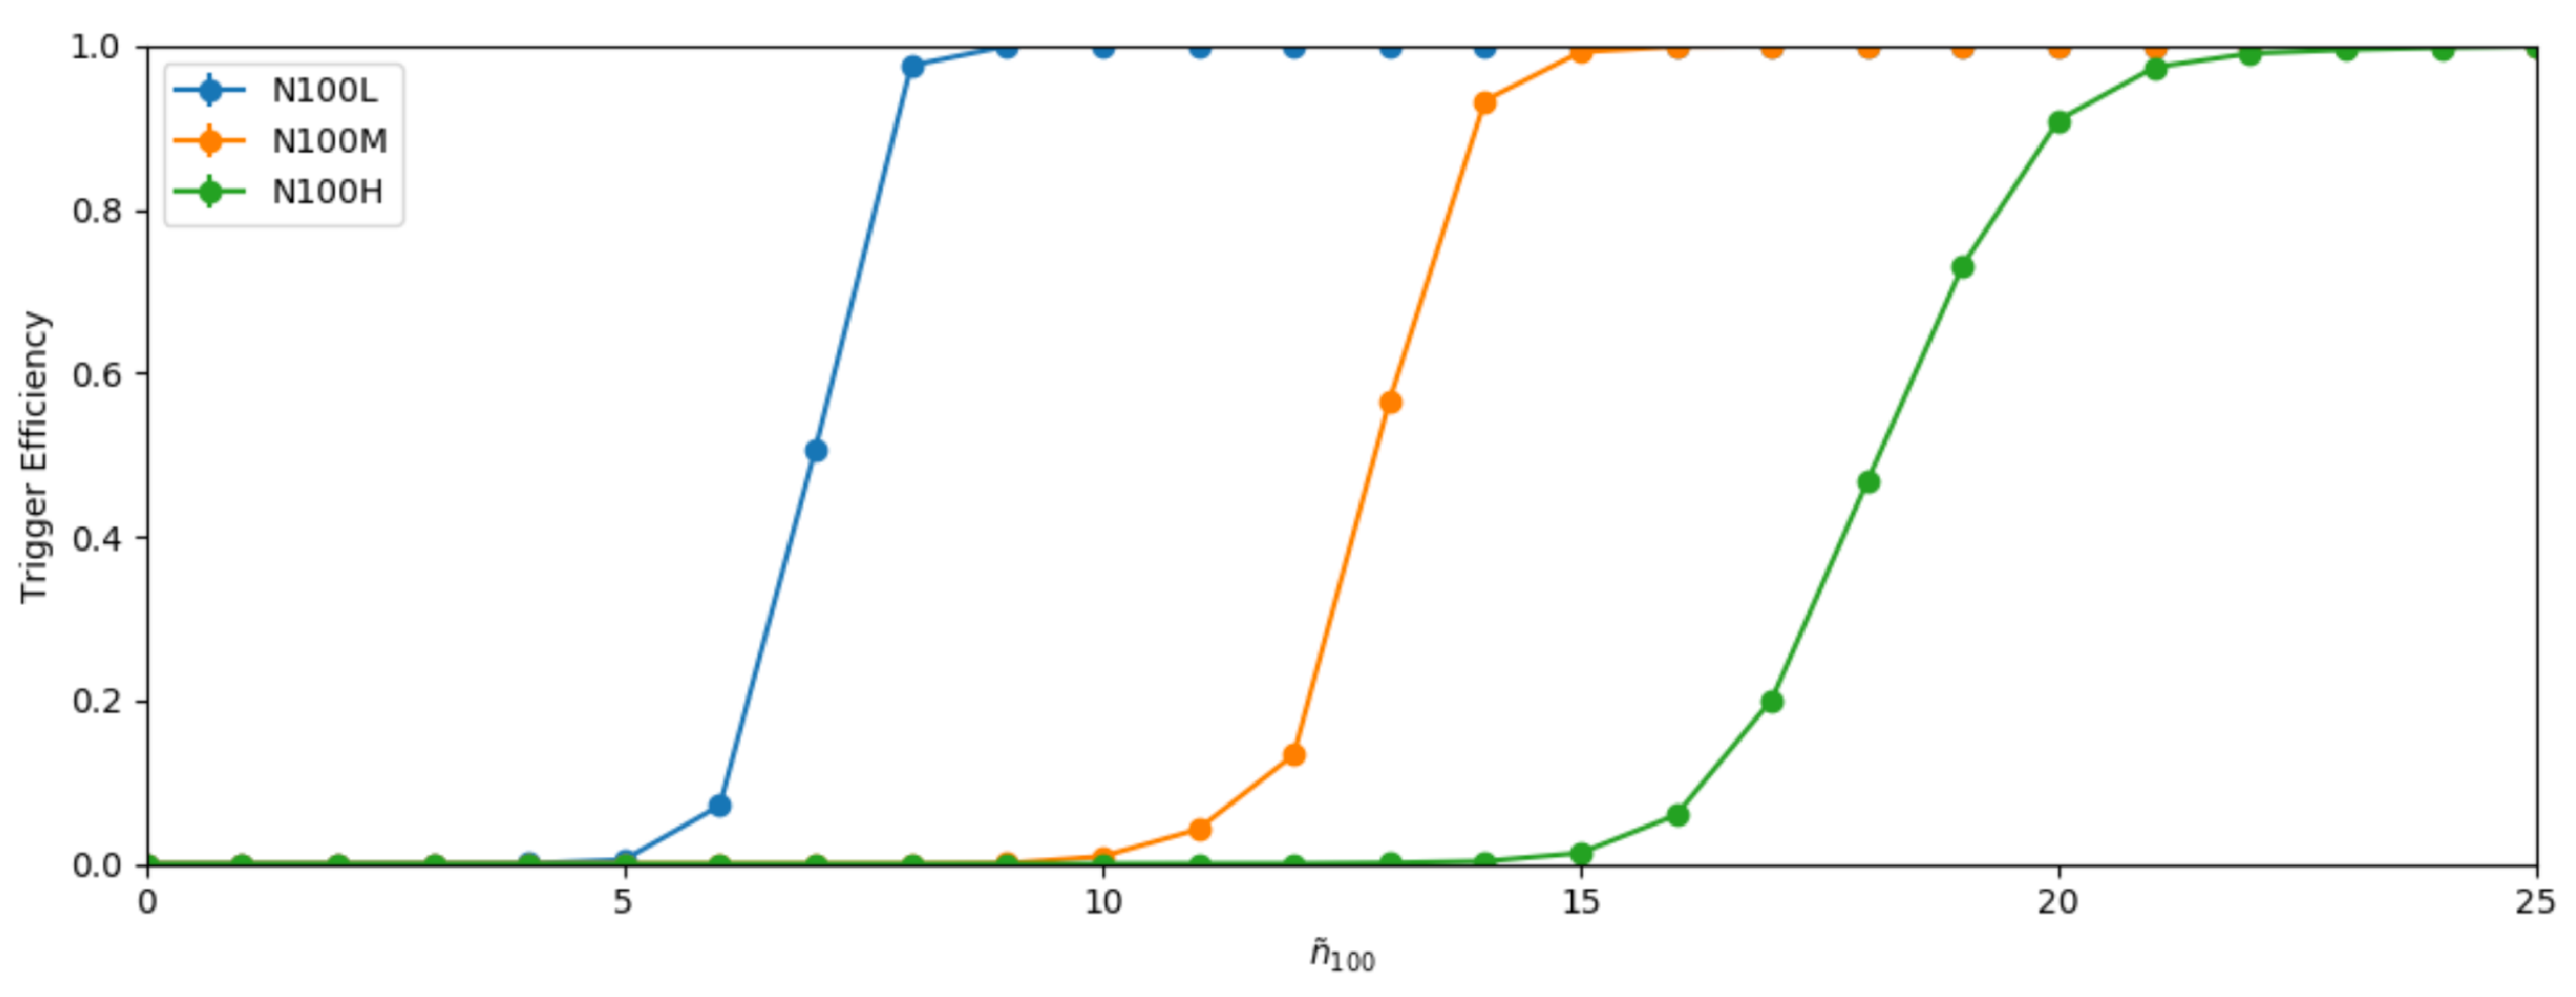
\includegraphics[width=\textwidth]{trigger_eff_plot2}
    \end{subfigure}
    \caption[Trigger Efficiecy, Before And After Threshold Changes]{
        (a) The trigger efficiency during the high threshold period for the
        N100 trigger as measured by nhit monitor, laserball, and TELLIE data,
        for N100L (left three curves) N100M (center three curves) and N100L
        (right three curves). (b) The trigger efficiency for the lower threshold
        data taking period from nhit monitor data.}
    \label{fig:trigeff_plots}
\end{figure}

The trigger efficiency for this analysis is defined to be the probability that
the detector will trigger on an event as a function of the number of ``in-time''
hits produced by that event.
Here, in-time hits is the effective maximum number of hits as seen by the analog
trigger system for an event.
For each event the in-time nhit, $\tilde{n}_{100}$, is well
estimated by the maximum number of hits in a 100\,ns window within the event.
Effects from the rise-time of trigger pulses and the limited band-width of the
trigger system are applied as corrections to that simple estimate.

The trigger efficiency is estimated in two different ways, using laserball
data, and using nhit monitor data.
Nhit monitor measurements of the trigger efficiency is discussed in ~\ref{sec:nhit_monitor}.
The laserball can measure the trigger efficiency because the same signal
that generates the light for the laserball also produces a trigger for
the DAQ\@.
So even if the light produced does not trigger the detector, the laserball signal
will ensure that the data is still readout.
So data was taken with a very low average light output from the laserball
and with that the trigger efficiency curve was measured near threshold.
The trigger efficiency curve produced by the nhit monitor and the laserball
data disagree by a small, but non-negligible amount, the
reason for the disagreement is not well-known, but the differences are taken
as a systematic uncertainty.
Figure~\ref{fig:trigeff_plots} shows the trigger efficiency curves
for nhit monitor, laserball, and TELLIE data.
Here, trigger efficiency is defined to be the probability that a raw-trigger
is emitted for a given event.

For data taken after the detector threshold change discussed in Sec~\ref{sec:dataset}
all methods agree that the trigger is 100\% efficient for $\tilde{n}_{100} > 10$;
only events with energy significantly below the analysis threshold 
will have a $\tilde{n}_{100} \le 10$, and so the discrepant
estimates of the trigger
efficiency do not have any effect on the solar analysis for the second trigger period.
For the first trigger period the trigger was not 100\% efficient until
$\tilde{n}_{100} \approx 23$, which is much closer to the analysis energy
threshold, and therefore uncertainties cannot be neglected.
Section~\ref{sec:systematics} discusses how the observed trigger efficiency
uncertainties were handled in the solar analysis.
